\documentclass[12pt]{article}
\usepackage{amsmath, amssymb, enumitem, fancyhdr, graphicx, libertine, nth,
  pgfplots, tikz, xcolor}
\pgfplotsset{compat=1.11}
\usetikzlibrary{decorations.pathreplacing}
\usetikzlibrary{patterns}
\usetikzlibrary{shadings}
\usepackage[margin=1in]{geometry}
\usepackage[libertine]{newtxmath}
\pagestyle{fancy}
\definecolor{solution-color}{HTML}{000080}
\chead{\emph{EC201 -- Problem Set 4 -- Solutions}}

% Define new topic command
\newcommand{\topic}[1]{\medskip\begin{center}\large\textsc{#1}\normalsize
  \end{center}}

% Define question counter:
\newcounter{question}[section]
\newcommand{\question}[1]{\refstepcounter{question}
  \subsubsection*{Question~\thequestion~-- #1}}

% Subquestions are enumerate with letters
\newenvironment{subquestions}{
  \begin{enumerate}[label=(\roman*)]}{\end{enumerate}}

\begin{document}

\topic{Elasticities}
\question{Cobb-Douglas Elasticities}
Your utility function for goods 1 and 2 is given by:
\[
  u\left( x_1,x_2 \right)=x_1^{\frac{1}{3}}x_2^{\frac{2}{3}}
\]
\begin{subquestions}
  \item Derive the demand functions $x_1\left( p_1,p_2,m \right)$ and $x_2\left(
    p_1,p_2,m \right)$.

    \textcolor{solution-color}{
      The $MRS$ is:
      \[
        MRS=-\frac{MU_1}{MU_2}=-\frac{\frac{1}{3}x_1^{\frac{1}{3}-1}x^{\frac{2}{3}}}{\frac{2}{3}x_1^{\frac{1}{3}}x^{\frac{2}{3}-1}}=-\frac{1}{2}\frac{x_2}{x_1}
      \]
      The optimality condition is to set $\left| MRS \right|=\frac{p_1}{p_2}$.
      From this we get $x_2=2x_1\frac{p_1}{p_2}$. Using this expression for
    $x_2$ in the budget constraint we can solve for $x_1$ to get the demand
    (same as on previous problems):
      \[
        x_1\left( p_1,p_2,m \right) = \frac{m}{3p_1}
      \]
      Then using this expression for $x_1$ in $x_2=2x_1\frac{p_1}{p_2}$ we can
      get:
      \[
        x_2\left( p_1,p_2,m \right) = \frac{2m}{3p_2}
      \]
    }
  \item Find the own-price elasticity of demand for good 1, $\varepsilon_1$.

    \textcolor{solution-color}{
      The formula for the own-price elasticity of demand for good 1 is:
    \[
      \varepsilon_1=\frac{\partial x_1\left( p_1,p_2,m \right)}{\partial p_1}
      \frac{p_1}{x_1\left( p_1,p_2,m
      \right)}
    \]
    The first term in the formula is the derivative of the demand function with respect to price. This is:
    \[
      \frac{\partial x_1\left( p_1,p_2,m \right)}{\partial p_1}
      = -\frac{m}{3p_1^2}
    \]
    Where you should recall that the derivative of $\frac{1}{x}$ is $-\frac{1}{x^2}$. We can use this in the rest of the formula:
  \[
      \varepsilon_1=\frac{\partial x_1\left( p_1,p_2,m \right)}{\partial p_1}
      \frac{p_1}{x_1\left( p_1,p_2,m
      \right)}=\left(-\frac{m}{3p_1^2}\right)\frac{p_1}{x_1\left( p_1,p_2,m \right)} = \left(-\frac{m}{3p_1^2}\right)\frac{p_1}{\frac{m}{3p_1}}=-1
    \]
    Every term cancels and we are left with the own-price elasticity of demand  being equal to -1.
  }
  \item Is good 1 an ordinary or Giffen good?

    \textcolor{solution-color}{
      Since $\varepsilon_1<0$ the good is ordinary.
  }
  \item Find the the cross-price elasticity of good 1 with respect to good 2,
    $\varepsilon_{12}$.

    \textcolor{solution-color}{
    Since $p_2$ doesn't show up in demand:
    \[
      \varepsilon_{12}=\frac{\partial x_1\left( p_1,p_2,m \right)}{\partial p_2}
      \frac{p_2}{x_1\left( p_1,p_2,m
      \right)}=0\times \frac{p_2}{x_1\left( p_1,p_2,m
      \right)}=0
    \]
  }
  \item Are the substitutes, complements, or neither?

    \textcolor{solution-color}{
      Since $\varepsilon_{12}=0$ they are neither.
  }
  \item Find the income elasticity of demand for good 1, $\eta_1$.

    \textcolor{solution-color}{
      The formula for the income elasticity is:
    \[
      \eta_1=\frac{\partial x_1\left( p_1,p_2,m \right)}{\partial m}
      \frac{m}{x_1\left( p_1,p_2,m
      \right)}
    \]
    The first term is:
    \[
      \frac{\partial x_1\left( p_1,p_2,m \right)}{\partial m}=\frac{1}{3p_1}
    \]
    We can use this in the rest of the formula:
    \[
      \eta_1=\frac{\partial x_1\left( p_1,p_2,m \right)}{\partial m}
      \frac{m}{x_1\left( p_1,p_2,m
      \right)}=
      \frac{1}{3p_1}\frac{m}{x_1\left( p_1,p_2,m \right)}=
      \frac{1}{3p_1}\frac{m}{\frac{m}{3p_1}}=1
    \]
    Every term cancels and we are left with an income elasticity of 1.
  }
  \item Is the good normal or inferior?

    \textcolor{solution-color}{
      Since $\eta_1=1$ the good is normal.
  }
\end{subquestions}
When finding the elasticities, do not just write down the answer. Show each
step in the calculation.

\question{Linear demand and Marginal Revenue}
The market demand curve for a good is given by:
\[
  D\left( p \right)=10-p
\]
\begin{subquestions}
  \item What is the own-price elasticity of demand at the following price and
    quantity pairs:
    \begin{enumerate}
      \item $p=4$ and $q=6$.
      \item $p=5$ and $q=5$.
      \item $p=6$ and $q=4$.
    \end{enumerate}
  Comment on whether demand is elastic, inelastic or unit elastic at each of
  these prices.

  \textcolor{solution-color}{
    For any price, the elasticity is:
    \[
      \varepsilon=\frac{dD\left( p \right)}{dp}\frac{p}{D\left( p \right)}=
      -1\times \frac{p}{10-p} = -\frac{p}{10-p}
    \]
    At the different prices we get:
    \begin{itemize}
      \item $\varepsilon\left( p=4 \right)=-\frac{2}{3}$ (Inelastic)
      \item $\varepsilon\left( p=5 \right)=-1$ (Unit elastic)
      \item $\varepsilon\left( p=6 \right)=-1.5$ (Elastic)
    \end{itemize}
  }
  \item Find the inverse demand curve, $p\left( q \right)$ for the demand
    curve above.

    \textcolor{solution-color}{
    The inverse demand function is:
    \[
      p\left( q \right)=10-q
    \]
    }
  \item Find the revenue function, $R\left( q \right)$ for a single firm
    selling to this market.

  \textcolor{solution-color}{
    The revenue function is:
    \[
      R\left( q \right)=p\left( q \right)q = \left( 10-q \right)q=10q-q^2
    \]
    }
  \item Find the marginal revenue function $MR\left( q \right)$.

  \textcolor{solution-color}{
    The marginal revenue function is:
    \[
      MR\left( q \right)=\frac{dR\left( q \right)}{dq}=10-2q
    \]
    }
  \item What is the marginal revenue at each of the price and quantity pairs in
    (i) above?
    \textcolor{solution-color}{
      \begin{itemize}
        \item $MR\left( q=6 \right)=-2$
        \item $MR\left( q=5 \right)=0$
        \item $MR\left( q=4 \right)=2$
      \end{itemize}
    }
  \item What does your finding in (v) tell us about the relationship between
    elasticity and marginal revenue?
    \textcolor{solution-color}{
      \begin{itemize}
        \item If demand is inelastic, marginal revenue is negative.
        \item If demand is elastic, marginal revenue is positive.
        \item If demand is unit elastic, marginal revenue is zero.
      \end{itemize}
    }
\end{subquestions}

\topic{Monopoly}
\question{Monopoly}
The (inverse) market demand for a good is given by $p\left( q \right)=130-q$
and there is a single producer with a cost function, $c(q) = 1600+10q+q^2$.
Find the equilibrium price, quantity, and profits for the monopolist.

    \textcolor{solution-color}{
      The monopolist's revenue function is:
      \[R\left( q \right)=p\left( q
      \right)q=\left( 130-q
    \right)q=130q-q^2\]
    The marginal revenue function is \[MR\left( q
    \right)=130-2q\]
    The marginal cost is \[MC\left( q \right)=10+2q\]
      Setting $MR\left( q \right)=MC\left( q \right)$ and solving for $q$:
      \[
        130-2q=10+2q \;\;\;\;\;\Longleftrightarrow\;\;\;\;\;
        4q=120\;\;\;\;\;\Longleftrightarrow\;\;\;\;\;
        q=30
      \]
      Using this in the demand curve we find that $p=130-30=100$.
      The profit for the monopolist is:
      \[
        \pi = p\times q - 1600 - 10q - q^2 = 100\times 30 - 1600 - 10\times 30
        - 30^2 = 3000 - 1600 - 300 - 900 =200
      \]
      So $q=30$, $p=100$ and $\pi=200$.
}

\question{Monopoly vs.~Perfect Competition with Linear Demand and Costs}
The inverse demand curve for a good is given by:
\[
  p\left( q \right)=10-q
\]
The cost function for the monopolist is:
\[
  c\left(  q\right)=2q
\]
\begin{subquestions}
  \item Derive the optimal price an quantity the monopolist will choose.

    \textcolor{solution-color}{
      The monopolist's revenue function is:
      \[
        R\left( q \right)=p\left( q \right)q = \left( 10-q \right)q=10q-q^2
      \]
      The marginal revenue is:
      \[
        MR\left( q \right)=10-2q
      \]
      The marginal cost is:
      \[
        MC\left( q \right)=2
      \]
      To find the optimal quantity, set $MR\left( q \right)=MC\left( q
      \right)$:
      \[
        10-2q=2 \;\;\;\;\Longleftrightarrow\;\;\;\;
        2q=8 \;\;\;\;\Longleftrightarrow\;\;\;\;
        q=4\
      \]
      The price is then found using the demand curve: $p=10-4=6$.
    }
  \item Confirm that the monopolist charges a mark-up over marginal cost of
    $\frac{1}{1-\frac{1}{\left| \varepsilon \right|}}$. You can use your
    answer in Q2 (i).

    \textcolor{solution-color}{
      The mark-up over marginal cost here is 3 (the monopolist charges 3 times
      the marginal cost).
      In Q2 (i) we found that $\varepsilon\left( p=6 \right)=-1.5$.
      So:
      \[
        \frac{1}{1-\frac{1}{\left| \varepsilon
        \right|}}=\frac{1}{1-\frac{1}{1.5}}=\frac{1}{1-\frac{2}{3}}=\frac{1}{\frac{1}{3}}=3
      \]
      So indeed the monopolist charges a mark-up over marginal cost of
      $\frac{1}{1-\frac{1}{\left| \varepsilon \right|}}$.
    }
  \item Find the profit the monopolist makes.

    \textcolor{solution-color}{
      The profit is $\pi=\left( p-AC \right)q=\left( 6-2 \right)\times
      4=16$.
    }

  \item Draw a diagram showing the following:
    \begin{itemize}
      \item The inverse demand curve.
      \item The marginal revenue curve.
      \item The marginal cost curve.
      \item The monopolist's price and quantity.
      \item The consumer surplus.
      \item The monopolist's profits.
      \item The deadweight loss.
    \end{itemize}
    The scaling of the diagram does not need to be exact. However, the
    lines/curves should have the correct shape.

  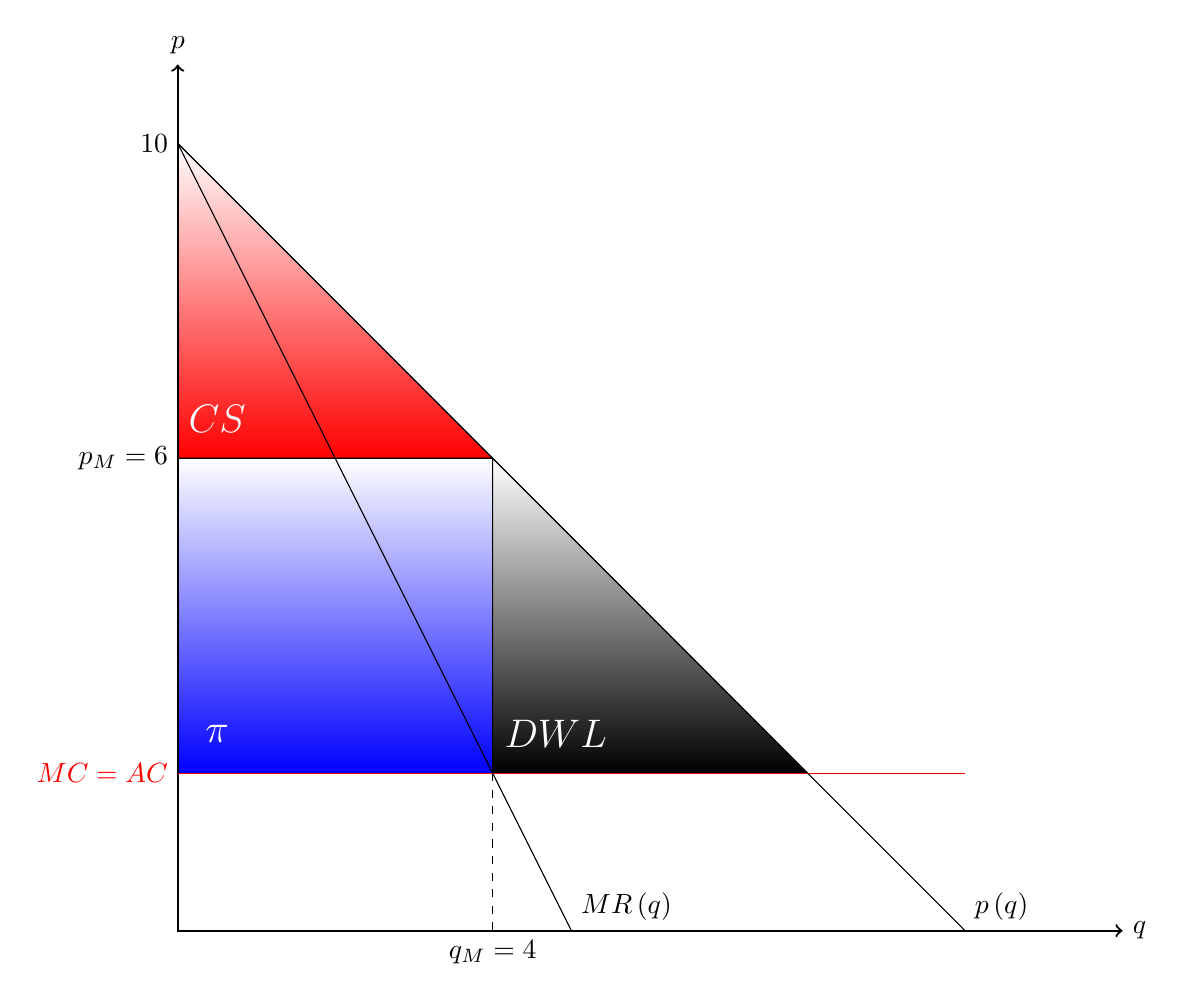
\begin{tikzpicture}
    \draw[top color=white,bottom color=red] (0,6) -- (4,6) -- (0,10) -- cycle;
    \draw (0.5,6.5) node[white] {\Large{$CS$}};
    \draw[top color=white,bottom color=blue] (0,2) -- (4,2) -- (4,6) -- (0,6)
    -- cycle;
    \draw (0.5,2.5) node[white] {\Large{$\pi$}};
    \draw[top color=white,bottom color=black] (4,6) -- (4,2) -- (8,2) -- cycle;
    \draw (4.8,2.5) node[white] {\Large{$DWL$}};
    \draw[thick,<->] (0,11) node[above] {$p$}--(0,0)--(12,0) node[right] {$q$};
    \draw (0,10) node[left] {$10$};
    \draw[-,red] (0,2) node[left, red] {$MC=AC$} (0,2)--(10,2);
    \draw[dashed,-] (0,6) node[left] {$p_M=6$} (0,6)--(4,6);
    \draw[dashed,-] (4,0) node[below] {$q_M=4$} (4,0)--(4,6);
    \draw (0,10)--(10,0);
    \draw (0,10)--(5,0);
    \draw (10,0) node[above right] {$p\left( q \right)$};
    \draw (5,0) node[above right] {$MR\left( q \right)$};
  \end{tikzpicture}
  \item What is the consumer surplus?

    \textcolor{solution-color}{
      To find the consumer surplus, we find the area of the triange:
      \[
        CS_M=\frac{1}{2}\times \left( 10-6 \right)\times 4 = 8
      \]
    }

  \item What is the deadweight loss, if any?

    \textcolor{solution-color}{
      To find the deadweight loss, we find the area of the triange:
      \[
      DWL_M=\frac{1}{2}\times \left( 6-2 \right)\times \left( 8-4 \right) = 8
      \]
    }
\end{subquestions}
Now assume the market was instead served by a large number of \textbf{perfectly
competitive} firms.
\begin{subquestions}
  \setcounter{enumi}{5}
  \item What would the price and quantity be? What profit would each of the
    firms make?

    \textcolor{solution-color}{
      The quantity occurs where $p=MC$. So $p=2$. The quantity demanded is then
      $q=10-p=10-2=8$.
      Since $MC=AC$, and $p=AC$, the profits would be zero.
    }
  \item Draw a diagram showing the following:
    \begin{itemize}
      \item The inverse demand curve.
      \item The marginal cost curve.
      \item The perfectly competitive price and quantity.
      \item The consumer surplus.
      \item The producer surplus.
    \end{itemize}

    \textcolor{solution-color}{
      There is zero producer surplus and zero deadweight loss.
    }

  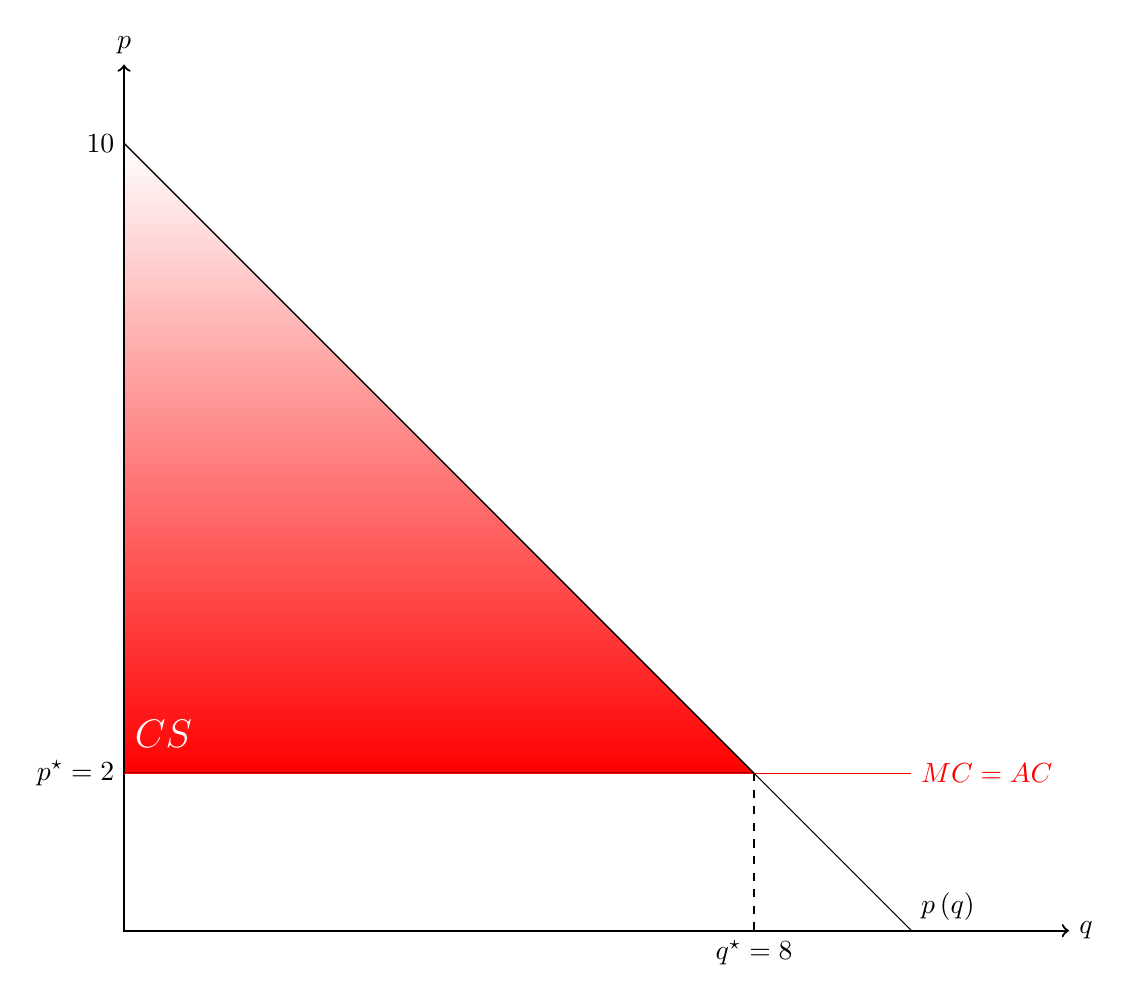
\begin{tikzpicture}
    \draw[top color=white,bottom color=red] (0,2) -- (8,2) -- (0,10) -- cycle;
    \draw (0.5,2.5) node[white] {\Large{$CS$}};
    \draw[thick,<->] (0,11) node[above] {$p$}--(0,0)--(12,0) node[right] {$q$};
    \draw (0,10) node[left] {$10$};
    \draw[-,red] (10,2) node[right] {$MC=AC$} (0,2)--(10,2);
    \draw (0,2) node[left] {$p^\star=2$};
    \draw[dashed,-] (8,0) node[below] {$q^\star=8$} (8,0)--(8,2);
    \draw (0,10)--(10,0);
    \draw (10,0) node[above right] {$p\left( q \right)$};
  \end{tikzpicture}

  \item What is the consumer surplus?

    \textcolor{solution-color}{
      The area of the triangle:
      \[
        CS^\star = \frac{1}{2}\left( 10-2 \right)\times 8=32
      \]
    }

  \item What is the producer surplus?

    \textcolor{solution-color}{
      $PS^\star=0$
    }

  \item What is the deadweight loss, if any?

    \textcolor{solution-color}{
      $DWL^\star=0$
    }

  \item How do each of price, quantity, profits, producer surplus, consumer
    surplus and deadweight loss compare between monopoly and perfect competition?

    \textcolor{solution-color}{
      \begin{itemize}
        \item  The monopolist charges a higher price
        \item The monopolist sells a lower quantity.
        \item The monopolist makes positive profits and the perfectly
          competitive firms make zero profits.
        \item The monopolist gets positive producer surplus and the perfectly
          competitive firms get zero producer surplus.
        \item The consumer surplus is larger under perfect competition.
        \item There is a deadweight loss in monopoly. There is no deadweight
          loss in perfect competition.
      \end{itemize}
    }
\end{subquestions}

\question{Natural Monopoly}
The inverse demand curve for a good is given by:
\[
  p\left( q \right)=10-q
\]
The cost function for the monopolist is:
\[
  c\left(  q\right)=9
\]
\begin{subquestions}
  \item Derive the optimal price an quantity the monopolist will choose.

    \textcolor{solution-color}{
      The marginal revenue function is $10-2q$. The marginal cost is zero.
      Therefore the optimal quantity is $q=5$ and the price is $p=5$.
    }
  \item Find the profit the monopolist makes.

    \textcolor{solution-color}{
      The profit is $p\times q - c\left( q \right) = 25 - 9=16$.
    }
  \item What is the consumer surplus?

    \textcolor{solution-color}{
      The consumer surplus is $\frac{1}{2}\left( 10-5 \right)\times 5=12.5$
    }
\end{subquestions}
Suppose the government introduced some regulation which forced the monopolist
to charge at marginal cost.
\begin{subquestions}
  \setcounter{enumi}{3}
  \item What would the new price, quantity and profits be?

    \textcolor{solution-color}{
       Since marginal cost is zero, price is zero. The quantity demanded will
       then be 10. The profits will be -9 because the firm will have zero
       revenue.
    }
  \item What is the consumer surplus?

    \textcolor{solution-color}{
      The consumer surplus is $\frac{1}{2}\times 10 \times 10 = 50$.
    }
\end{subquestions}
Suppose the government introduced some regulation which forced the monopolist
to charge a price such that it makes zero profits overall.
\begin{subquestions}
  \setcounter{enumi}{5}
  \item What would the price, quantity and profits be?

    \textcolor{solution-color}{
      We set average cost equal to price: $AC\left( q \right)=p\left( q
      \right)$.
      So:
      \begin{align*}
        \frac{9}{q} & =10-q \\
        9 &=10q - q^2 \\
        q^2 - 10q + 9 &= 0 \\
        \left( q-1 \right)\left( q-9 \right)&=0
      \end{align*}
      So $AC\left( q \right)$ intersects $p\left( q \right)$ at 1 and 9. We are
      trying to make consumer surplus as big as possible so we should choose
      $q=9$. $q=1$ makes profits zero but the consumer surplus will be small.
      The price with $q=9$ is then $p=1$. The profits are zero.
    }
  \item What is the consumer surplus?

    \textcolor{solution-color}{
      \[
        CS=\frac{1}{2}\times \left( 10-1 \right)\times 9 = 40.5
      \]
    }
\end{subquestions}
There are three possible policies the government can pursue, the outcomes of
which you have solved for above:
    \begin{itemize}
      \item No regulation.
      \item Forcing the monopolist to charge at marginal cost.
      \item Forcing the monopolist to charge a price such that it makes zero
        profits.
    \end{itemize}
\begin{subquestions}
  \setcounter{enumi}{7}
  \item Which policy maximizes consumer surplus?
    \textcolor{solution-color}{
      The $p=MC$ policy maximizes consumer surplus ($CS=50$).
    }
  \item Which policy maximizes consumer surplus \emph{plus} profits?
    \textcolor{solution-color}{
      The sum of consumer surplus in each case is:
      \begin{enumerate}
        \item 16 + 12.5 = 28.5
        \item 50 - 9 = 41
        \item 0 + 40.5 = 40.5
      \end{enumerate}
      So charging $p=MC$ actually makes the largest surplus plus profits (but
      the monopolist will not be very happy with this arrangement).
    }
\end{subquestions}

\question{Two-Period Monopoly with an Experience Good}
Consider the following model of a two-period monopolist selling an
\emph{experience good}. The inverse market demand in the first period is
\[
  p\left( q_1 \right) =10-q_1
\]
In the second period the demand is:
\[
  p\left( q_2 \right) = 10+\frac{q_1}{2}-q_2
\]
The amount the monopolist sells in the second period depends on how much the
monopolist sold in the first period. The amount the monopolist sold in the
first period shifts out the second period demand curve (raises the vertical
intercept). The monopolist's cost function is $c\left( q_1,q_2 \right)=0$.
\begin{subquestions}
  \item If the monopolist was unaware he was selling an experience good and
    simply maximized profits in each period, what would his total profits be?

  \textcolor{solution-color}{
    $MC$ here is zero so to maximize profits the monopolist will set $MR=0$.
    The marginal revenue in period 1 is $MR_1=10-2q_2$. Setting this equal to zero
  yields $q_1=5$. This gives $p_1 =5$.}

  \textcolor{solution-color}{
  Given $q_1=5$, in the second period demand becomes $p_2 = 12.5-q_2$. Marginal
  revenue is period 2 is then $MR_2=12.5-2q_2$.  setting $MR_2=0$ yields
  $12.5-2q_2=0$, so $q_2 = 6.25$. Then $p_2=6.25$. Thus total profits are $25+
  \frac{625}{16} = 64.0625$.
}
  \item If the monopolist knows the way the demand curves depend on both
    quantities, write down his profit function for both periods. This should be
    a function of $q_1$ and $q_2$ only.

  \textcolor{solution-color}{
    The profit function is:
    \begin{align*}
      \pi\left( q_1,q_2 \right) &= q_1(10-q_1) + q_2(10+\frac{q_1}{2}-q_2) \\
      &= 10q_1 - q_1^2 + 10q_2 + \frac{q_1q_2}{2} - q_2^2
    \end{align*}
  }
  \item Solve for the optimal prices and quantities by maximizing the profit
    function you wrote down above. Remember that maximizing a function of two
    variables requires setting both partial derivatives equal to 0 and solving
    the system of equations. Does the monopolist offer a low introductory
    price?

  \textcolor{solution-color}{
The setting the partial derivatives with respect to $q_1$ and $q_2$ equal to
zero:
\begin{eqnarray*}
  \frac{\partial \pi}{\partial q_1} &=&10 -2q_1 +\frac{q_2}{2} =0 \\
  \frac{\partial \pi}{\partial q_2} &=&10+\frac{q_1}{2} -2q_2 =0
\end{eqnarray*}
If we solve these equations, we find that $p_1 = \frac{10}{3}$, $p_2 =
\frac{20}{3}$, $q_1 = \frac{20}{3}$ and $q_2 =\frac{20}{3}$. Thus, the
monopolist offers a lower introductory price in the first period, and then
raises it considerably in the second period.
  }
  \item Compare the profits from parts (i) and (iii). Is the monopolist better
    off in (i) or (iii)?

  \textcolor{solution-color}{
Plugging in the prices and quantities from (iii) we find that profits are $\frac{200}{3}$. Thus, the monopolist enjoys larger profits by charging the lower price in the first period to increase demand.
}
\end{subquestions}

\end{document}
